% Szenarien und Annahmen

\section{Auswertung bestehender Literatur und Einordnung der Arbeit}\label{chap:Literatur}

In diesem Kapitel erfolgt eine Metaanalyse relevanter Studien.
Dabei liegt der Fokus auf den getroffenen Annahmen der Studien zur Elektromobilität.
Bei den Studien, die sich explizit mit den Auswirkungen der Elektromobilität auf die Verteilnetze beschäftigen, wird ein weiterer Fokus auf die verwendete Methodik und Ergebnisse gelegt.


\subsection{Literatur Metaanalyse}\label{chap:Metaanalyse}

Aufgrund der zunehmenden Marktdurchdringung der Elektromobilität rückt die Frage der Rückwirkungen der Ladevorgänge auf die Stromnetze vermehrt in den Vordergrund.
Sind die Auswirkungen heutzutage noch klein, so kann ein stark steigender Markthochlauf auch starken Einfluss auf die Netzlast haben.


\subsubsection{Fahrzeughochlauf}

Die tatsächliche Anzahl von \glspl{EPKW} bildet die wichtigste Einflussgröße auf die Höhe der Rückwirkungen auf das Stromnetz ab.
Neben der Anzahl an Fahrzeugen haben auch die technischen Parameter der einzelnen Fahrzeugklassen einen starken Einfluss.
Die technischen Parameter der Fahrzeuge können \autoref{chap:EMob_Szenarien} entnommen werden und sind nicht Teil der Metaanalyse.

\begin{figure}[H]
    \centering
    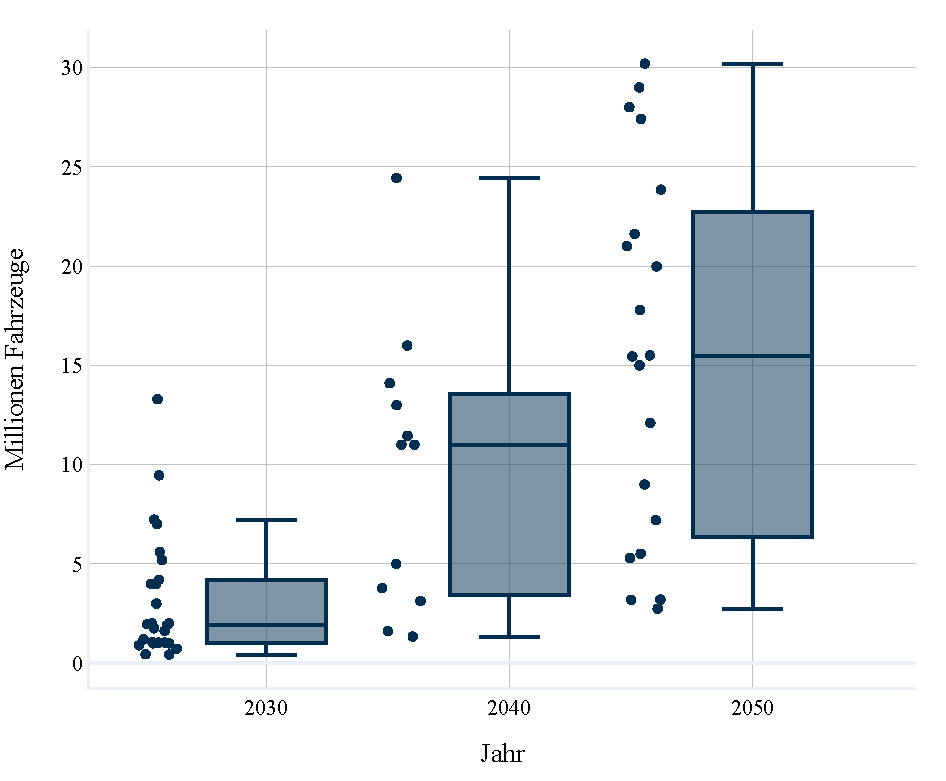
\includegraphics[width=\textwidth]{Bilder/RampUp-BEV-MA}
    \caption{Szenarienvergleich des Fahrzeugbestands von BEV bis zum Jahr \num{2050}}\label{fig:RampUpBEV}
\end{figure}

In \autoref{fig:RampUpBEV} sind die Annahmen der betrachteten Studien zum Fahrzeugbestand von \glspl{BEV} bis zum Jahr \num{2050} als Box-Plot dargestellt.
Die zugrundeliegenden Daten finden sich im Anhang in \autoref{tab:RampUpBEV}.
Trotz einer starken Streuung zeigt sich bis \num{2050} eine klare Zunahme im Bestand.
Der Median liegt 2030 noch bei \SI{1.9}{\MioStk}, steigt bis \num{2040} auf \SI{11.0}{\MioStk} und erreicht \num{2050} \SI{15.5}{\MioStk}.
Die starke Streuung lässt sich zum einen durch den unterschiedlichen Fokus der verschiedenen Studien und zum anderen durch den langen Zeithorizont und die damit verbundene Unsicherheit erklären.
In einzelnen Szenarien werden hohe Elektrifzierungsquoten angenommen und das Einhalten des \SIrange[range-phrase=~{--}~]{80}{95}{\percent}-Ziels des Klimaschutzplans \num{2050} vorausgesetzt, während andere Szenarien eine Fortschreibung der aktuellen Entwicklungen (\gls{BAU}) untersuchen.
So handelt es sich beispielsweise bei dem oberen Ausreißer im Jahr 2030 um das Elektrifizierungs-Szenario der dena-Leitstudie \glqq Integrierte Energiewende\grqq \cite{DEAGH2018}.
Hierbei handelt es sich um ein Szenario, welches hohe Elektrifizierungsquoten annimmt und als Leitlinie die Einhaltung des  \SIrange[range-phrase=~{--}~]{80}{95}{\percent}-Ziels setzt.\medskip

Neben dem Hochlauf an \glspl{BEV}, ist auch mit einem starken Hochlauf bei den \glspl{PHEV} zu rechnen.
Da ein Großteil der Fahrten von \glspl{PKW} eine Strecke von \SI{50}{\km} nicht überschreiten, können viele dieser Fahrten auch von \glspl{PHEV} batterieelektrisch zurückgelegt werden. \cite{Agora2019}
%Unterschiede gibt es jedoch in der maximalen Ladeleistung der Fahrzeugklassen.
%So werden \glspl{BEV} \num{2050} maximale Ladeleistungen von bis zu \SI{350}{\kw} aufweisen, während die maximale Ladeleistung von \glspl{PHEV} mit bis zu \SI{120}{\kw} deutlich geringer ausfällt. \cite{Kaul2019}

\begin{figure}[H]
    \centering
    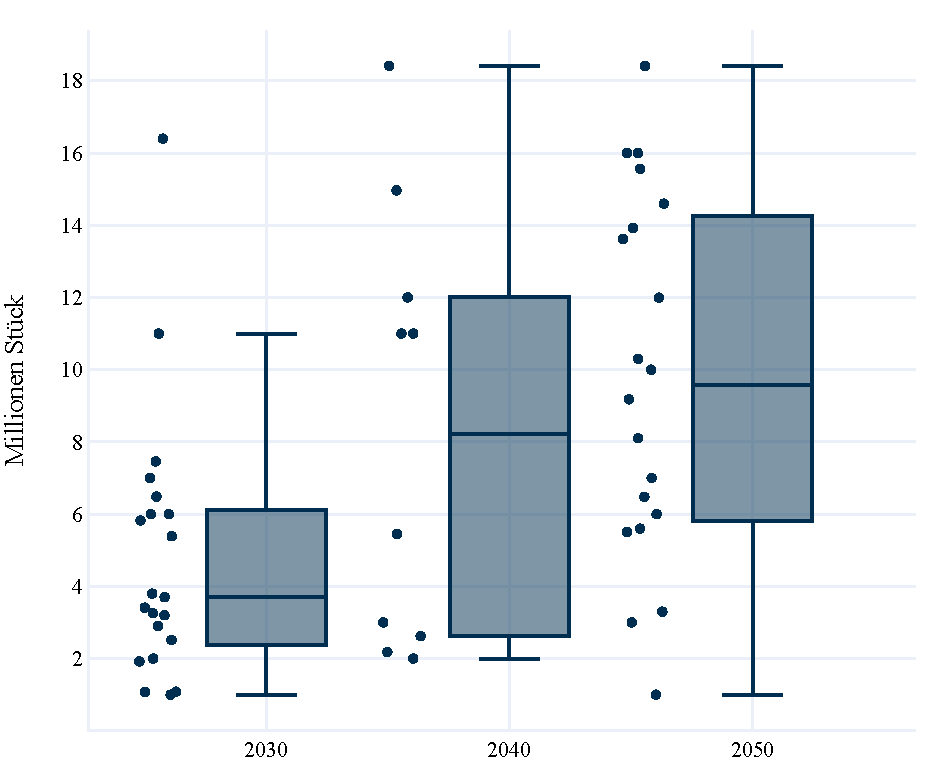
\includegraphics[width=\textwidth]{Bilder/RampUp-PHEV-MA}
    \caption{Szenarienvergleich des Fahrzeugbestands von PHEV bis zum Jahr \num{2050}}\label{fig:RampUpPHEV}
\end{figure}

\autoref{fig:RampUpPHEV} zeigt die Annahmen der betrachteten Studien zum Fahrzeugbestand von \glspl{PHEV} bis zum Jahr \num{2050} als Box-Plot.
Die zugrundeliegenden Daten finden sich im Anhang in \autoref{tab:RampUpPHEV}.
Bei \glspl{PHEV} liegt der Anstieg im Fahrzeugbestand anfangs sogar höher als bei \glspl{BEV}.
So liegt der Median 2030 bereits bei \SI{3.7}{\MioStk}.
Anschließend fällt der Fahrzeugbestand von \glspl{PHEV} hinter den der \glspl{BEV} zurück.
Bis \num{2040} steigt dieser auf \SI{8.2}{\MioStk} und \num{2050} auf \SI{9.6}{\MioStk}.
Je nach Studie und Szenario sinkt der Fahrzeugbestand nach \num{2040} sogar wieder, da zur Erreichung der Klimaziele oder aus ökonomischen Gründen der Umstieg auf \glspl{BEV} sinnvoller ist.

\begin{figure}[H]
    \centering
    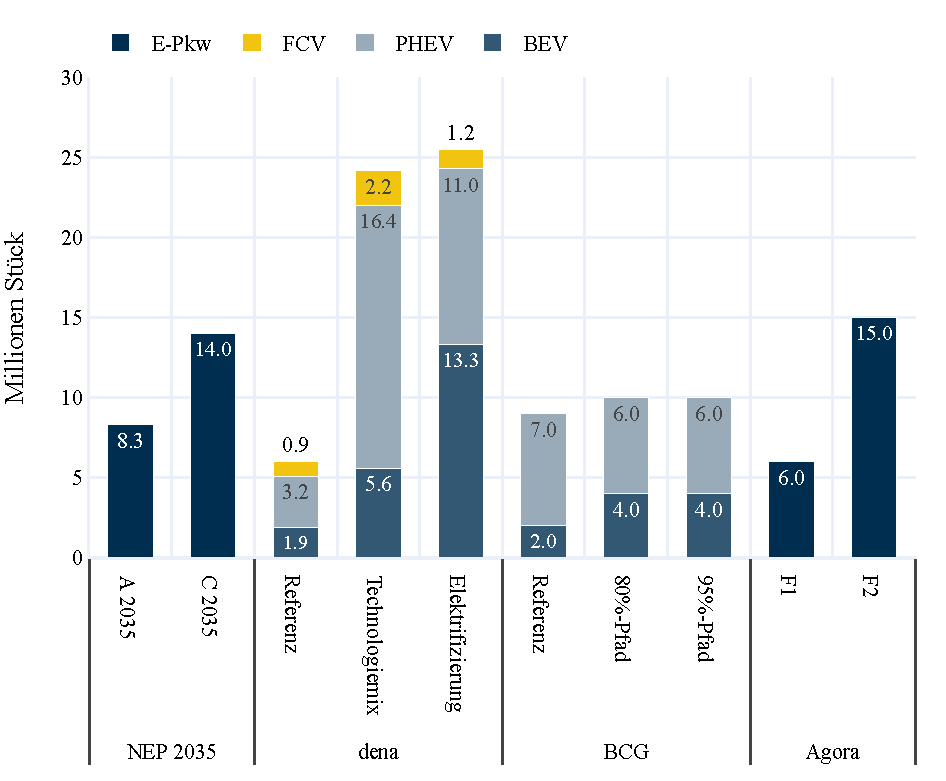
\includegraphics[width=\textwidth]{Bilder/RampUp-2030-Focus-MA}
    \caption{Fahrzeughochlauf alternativer Antriebstechnologien je Studie und Szenario bis zum Jahr \num{2030}}\label{fig:RampUp2030}
\end{figure}

Von den betrachteten Studien quantifizieren drei Studien den Netzausbaubedarf auf Verteilnetzebene und besitzen somit einen Vergleichswert zu der vorliegenden Arbeit und werden vertieft betrachtet.
Hierzu zählen die dena-Leitstudie \glqq Integrierte Energiewende\grqq{} \cite{DEAGH2018}, die BCG Studie \glqq Klimapfade für Deutschland\grqq{} \cite{BCG2018} und die Agora Studie \glqq Verteilnetzausbau für die Energiewende\grqq{} \cite{Agora2019}.
\autoref{fig:RampUp2030} zeigt den Fahrzeughochlauf verschiedener alternativer Antriebstechnologien im Verkehrssektor bis \num{2030} je Studie und Szenario.
Als Referenz wurden die konservativsten und progressivsten Annahmen des Netzentwicklungsplans \numrange[range-phrase=~{--}~]{2021}{2035} \cite{BNetzA2020} hinzugefügt.
Zu beachten ist hierbei, dass sich der Netzentwicklungsplan im Gegensatz zu den anderen Studien auf das Stützjahr \num{2035} bezieht.
Es wird erneut deutlich, dass sich der Markthochlauf je Studie und Szenario teils erheblich unterscheidet.
Grund hierfür sind nicht nur unterschiedliche Zielsetzungen der Studien, sondern auch verschiedene Modellgrundlagen und Annahmen.
So spannen sowohl die dena-Leitstudie als auch die BCG Studie einen Szenariorahmen für die Erreichung der Klimaschutzziele bis \num{2050} auf.
Dennoch liegt der Fahrzeugbestand alternativer Antriebstechnologien in den Klimaschutzszenarien \glqq Technologiemix\grqq{} und \glqq Elektrifizierung\grqq{} der dena-Leitstudie im Jahr 2030 mehr als doppelt so hoch als in den vergleichbaren Szenarien \glqq \SI{80}{\percent}-Pfad\grqq{} und \glqq \SI{95}{\percent}-Pfad\grqq{} der BCG Studie.
Beide Studien betrachten die Erreichung der Klimaschutzziele über alle relevanten Sektoren.
Hierbei bewertet die BCG Studie den Verkehrssektor als deutlich unelastischer als die dena-Leitstudie, wodurch im Jahr \num{2030} eine große Diskrepanz zwischen den Szenarien entsteht.\medskip

Demgegenüber definiert die Agora Studie feste Markthochläufe und ermittelt auf Grundlage dieser den nötigen Netzausbaubedarf in Abhängigkeit verschiedener Ladestrategien und -leistungen.
Die angenommenen Markthochläufe basieren in den \textit{F}-Szenarien auf einer Fortschreibung des aktuellen Verkehrsverhaltens bei einer Antriebswende und in dem \textit{M}-Szenario (s. \autoref{fig:RampUp2050}) auf einer Mobilitätswende.

\begin{figure}[H]
    \centering
    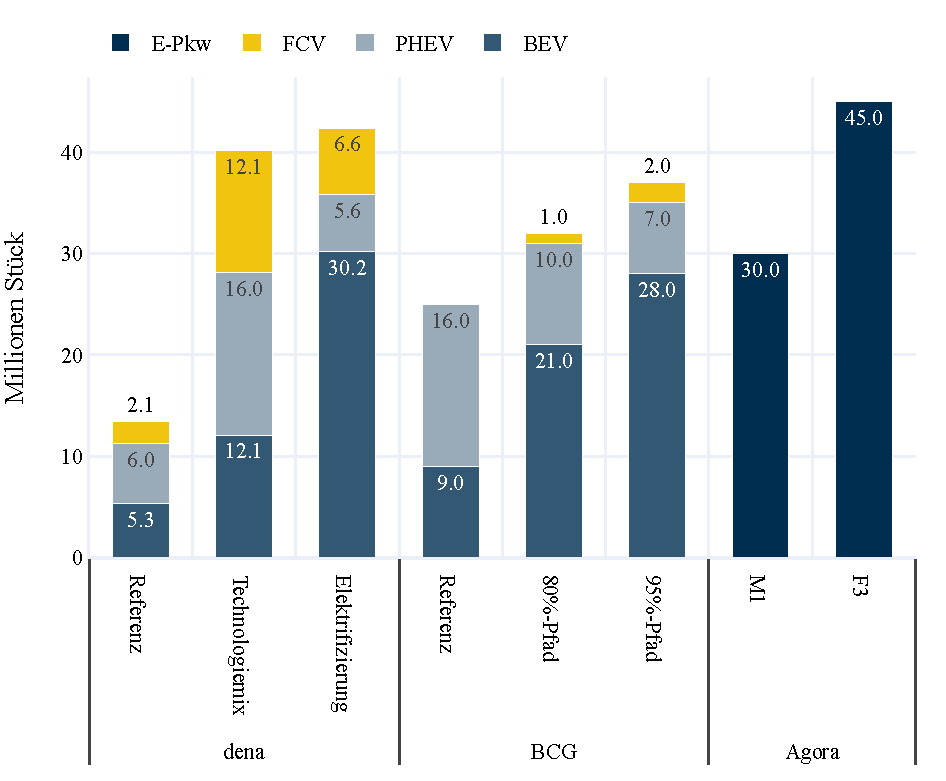
\includegraphics[width=\textwidth]{Bilder/RampUp-2050-Focus-MA}
    \caption{Fahrzeughochlauf alternativer Antriebstechnologien je Studie und Szenario bis zum Jahr \num{2050}}\label{fig:RampUp2050}
\end{figure}

In \autoref{fig:RampUp2050} findet sich der Fahrzeughochlauf verschiedener alternativer Antriebstechnologien im Verkehrssektor bis \num{2050} je Studie und Szenario.
Im Gegensatz zum Markthochlauf bis \num{2030} liegen die Markthochlaufzahlen bis \num{2050} in allen Studien auf einem ähnlichen Niveau.
Dennoch liegen die Zahlen der BCG-Szenarien unter denen der dena-Leitstudie.
Der Grund hierfür ist, dass die Erreichung der Klimaschutzziele in der BCG Studie stärker in die Sektoren Energie, Haushalte, \gls{GHD} und Industrie verlagert wurden.
Beide Studien sind sich jedoch einig, dass zum Erreichen der Klimaschutzziele der Markthochlauf alternativer Antriebstechnologien im Verkehrssektor gegenüber dem jeweiligen Referenz-Szenario (\gls{BAU}) deutlich angehoben werden muss.


\subsubsection{Methodik der zur Untersuchung der Verteilnetze}

{\color{red} TODO}

Die Kosten für den Netzausbau auf Verteilnetzebene in Deutschland werden von drei Studien untersucht.
Hierzu zählen die dena-Leitstudie \glqq Integrierte Energiewende\grqq{} \cite{DEAGH2018}, die BCG Studie \glqq Klimapfade für Deutschland\grqq{} \cite{BCG2018} und die Agora Studie \glqq Verteilnetzausbau für die Energiewende\grqq{} \cite{Agora2019}.

\begin{figure}[H]
    \centering
    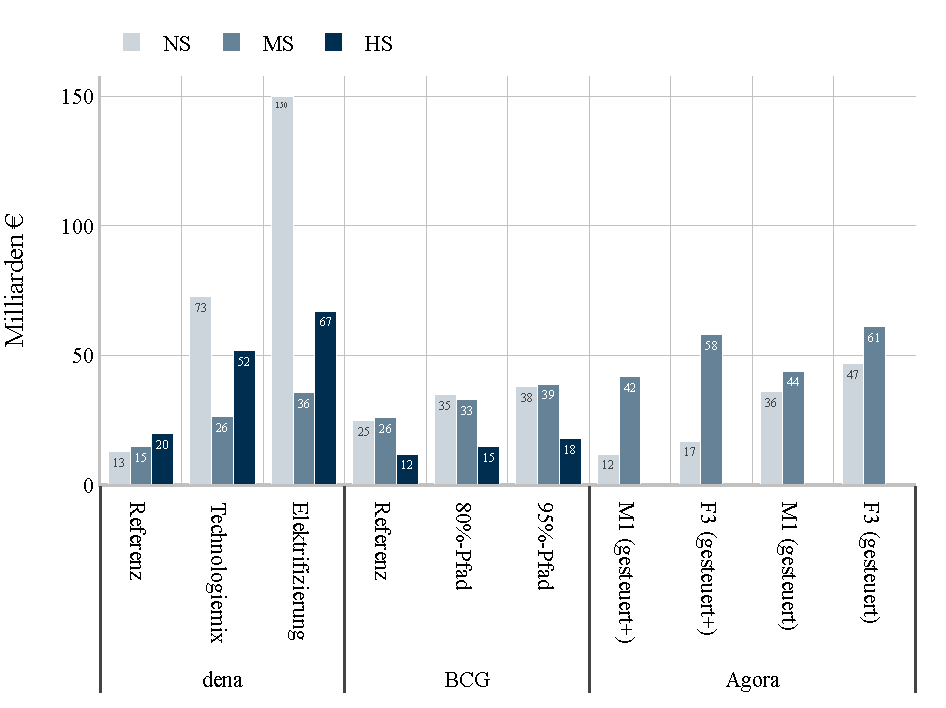
\includegraphics[width=\textwidth]{Bilder/DS-CAPEX-MA}
    \caption{Investitionsbedarf in die Verteilnetze bis zum Jahr \num{2050} je Spannungsebene}\label{fig:DSCAPEXMeta}
\end{figure}

In \autoref{fig:DSCAPEXMeta} finden sich die Ergebnisse der Studien für den Investitionsbedarf in die Verteilnetze bis zum Jahr \num{2050} aufgeteilt auf die drei Spannungsebenen \gls{NS}, \gls{MS} und \gls{HS}.
Deutlich wird hierbei, dass die dena-Leistudie die mit Abstand höchsten Kosten für den Netzausbau auf \gls{NS}- und \gls{HS}-Ebene ermittelt.
Die Agora Studie untersucht hingegen die Netzausbaukosten nicht auf der \gls{HS}-Ebene, ermittelt jedoch die höchsten Ausbaukosten aller Studien auf der \gls{MS}-Ebene.
Ein direkter Vergleich der Ergebnisse ist jedoch nur bedingt möglich, da die drei Studien unterschiedliche Grundsätze für ihre Szenarien und die Bestimmung des Netzausbaubedarfs ansetzen.\medskip

Teilweise erklären lassen sich diese Unterschiede zwischen den Ergebnissen der Studien durch die verschiedenen Annahmen zum Hochlauf an erneuerbaren Erzeugerkapazitäten und neuen Verbrauchern.
Dabei unterscheiden sich die Studien jedoch maximal um einen Faktor \num{1.5} bei den Erzeugerkapazitäten und neuen Verbrauchern, während die Investitionskosten in den ambitionierten Szenarien auf der \gls{NS}-Ebene sogar um den Faktor \num{4} auseinander liegen.
Ein deutlicher Unterschied entsteht durch die Annahme der dena-Leitstudie, dass eine Steuerung der Ladevorgänge von neuen Verbrauchern nicht stattfindet.
Stattdessen geht die Studie davon aus, dass die zusätzliche Last durch \glspl{EPKW} und \glspl{WP} gleichzeitig mit der bisherigen Spitzenlast auftritt und der auslegungsrelevante Starklastfall somit deutlich erhöht wird.
Im Gegensatz zur dena-Leitstudie wird in der BCG-Studie von einem gesteuerten Laden der neuen Verbraucher ausgegangen.
Dabei wird bei \glspl{WP} ein zweistündiger Warmwasserspeicher unterstellt, wodurch ein ebenso langer Starklastfall überbrückt werden kann.
\SI{80}{\percent} der \glspl{EPKW} reagieren auf Strommarktsignale und werden nur geladen, wenn der \gls{SOC} auf weniger als \SI{50}{\percent} fällt oder eine lange Fahrt ansteht.
Bei der Agora Studie wird ein starker Fokus auf den Einfluss von unterschiedlichen Ladestrategien auf den Netzausbaubedarf gelegt und ein konsequent netzdienliches Verhalten von \gls{EPKW} gesetzt, indem eine Residuallastglättung innerhalb eines Netzgebietes angestrebt wird (gesteuert).
Zusätzlich wurde ein erweitertes netzdienliches Ladekonzept (gesteuert\Plus) untersucht, welches zusätzlich die Verschiebung der Ladevorgänge über mehrere Standzeiten und eine Kappung von Lastspitzen erlaubt.\medskip

Die starken Differenzen zwischen den Ergebnissen der Studien lassen sich also vermutlich zu einem erheblichen Teil durch die unterschiedlichen Annahmen zur Steuerbarkeit von neuen Verbrauchern erklären.
Dies macht deutlich, welche Bedeutung der Flexibilisierung von Verbrauchern mit hohen Leistungsklassen zukommen sollte


\subsubsection{Abgrenzung zur bestehenden Literatur}

{\color{red} TODO}

In der ausgewerteten Literatur werden die Auswirkungen einer zunehmenden Netzintegration von \glspl{EPKW} auf die Verteilnetze in Deutschland bereits in ihrer Gesamtheit betrachtet.
In dieser Arbeit werden ergänzend die Auswirkungen auf sechs Netzklassen untersucht, welche jeweils stark unterschiedliche Charakteristiken besitzen und grob in die Kategorien \gls{PV}-, Wind- bzw- Last-dominiert eingeteilt werden können.
Hierbei wird der Einfluss verschiedener netzdienlicher Ladestrategien untersucht und der Erfolg von präventiven und aktiven Ansätzen miteinander verglichen.\medskip

Weiterhin erfolgt die Modellierung der \glspl{EPKW} und der entsprechenden Ladeinfrastruktur in einer sehr hohen Detailtiefe.
So werden insgesamt vier Hochlaufszenarien und zwei Szenaretten betrachtet.
Auf diese Weise werden unterschiedliche Durchdringungstiefen mit \glspl{EPKW} abgebildet und der Einfluss einer Variation der Eingangsparameter der \glqq Aufteilung der Fahrzeugflotte in verschiedene Farzeugklassen\grqq , sowie der \glqq Verfügbarkeit von Ladeinfrastruktur am Arbeitsplatz\grqq{} untersucht.


